\documentclass[12pt,a4paper]{report}
\usepackage[utf8]{inputenc} % un package
\usepackage[T1]{fontenc} % un second package
\usepackage[francais]{babel} % un troisième package
\usepackage{color} % Package de la couleur
\usepackage{verbatim}
\usepackage{moreverb}
\usepackage{amsmath}
\usepackage{amsfonts}
\usepackage{amssymb}
\usepackage{graphicx}
\usepackage[top=2cm, bottom=2cm, left=2cm, right=2cm]{geometry}
\author{IMA World Health Web Developer Team}
\title{
\includegraphics[width=12cm]{ima.png} \\BASIC HOSPITAL INFORMATION MANAGEMENT APPLICATION\\ (BHIMA) \\ Manuel d'utilisation}

\begin{document}
%Page de garde
\maketitle 
\chapter{Présentation}
\section{Accès au système}
\large{Pour accéder au système, la première de chose à faire est de lancer un navigateur web, en suite saisir l'adresse web de server dans la barre d'adresse du navigateur.}

La première interface de l'application est un formulaire qui demande à chaque utilisateur de pouvoir fournir son login, son mot de passe mais aussi de spécifier  le projet dont il sont assigné, comme le montre le formulaire ci-dessous.
\begin{figure}[h]
\begin{center}
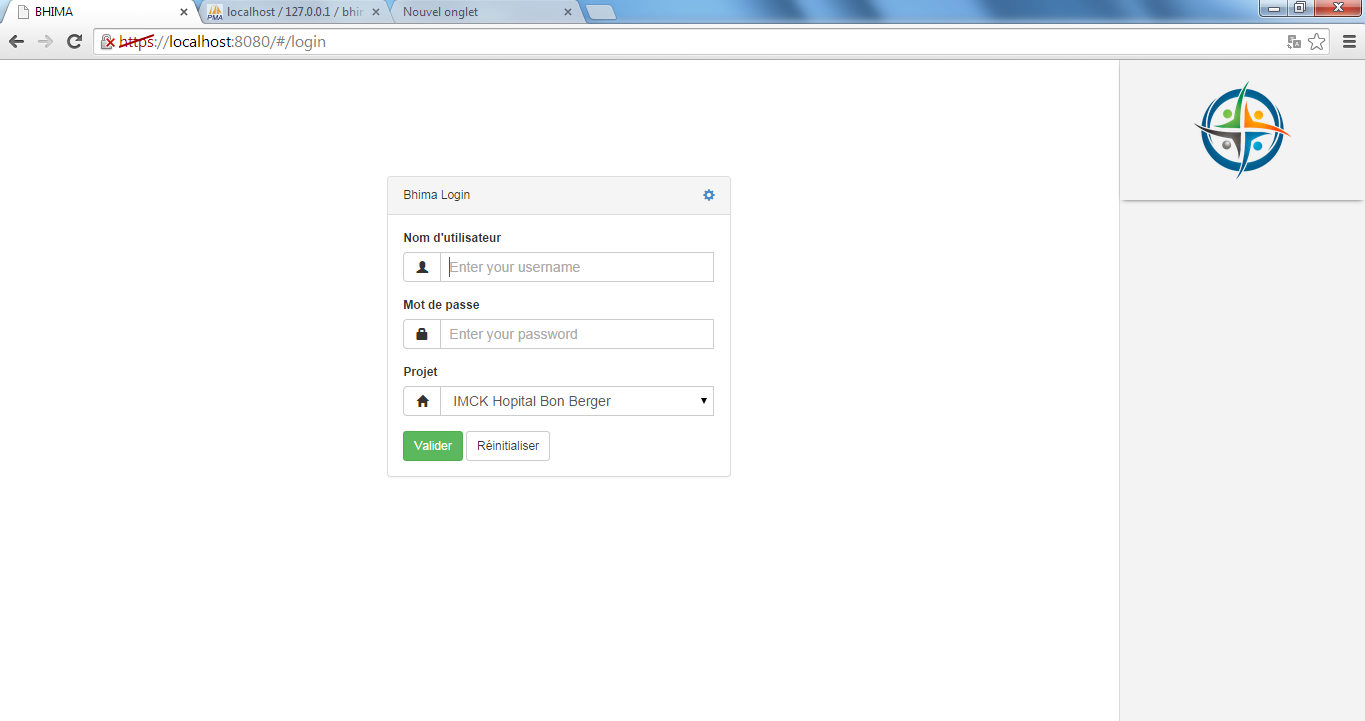
\includegraphics[width=12cm]{pic/login.png}
\end{center}
\caption{Page d'identification et authentification des utilisateurs}
\label{Page d'identification et authentification des utilisateurs}
\end{figure}
\\ L'accès au système n'est garanti que pour ceux qui possèdent un compte utilisateur, si l'utilisateur s'est authentifié alors il sera dirigé vers l'interface principale de l'application qui se présente de la manière suivante.
\newpage
\begin{figure}[h]
\begin{center} 
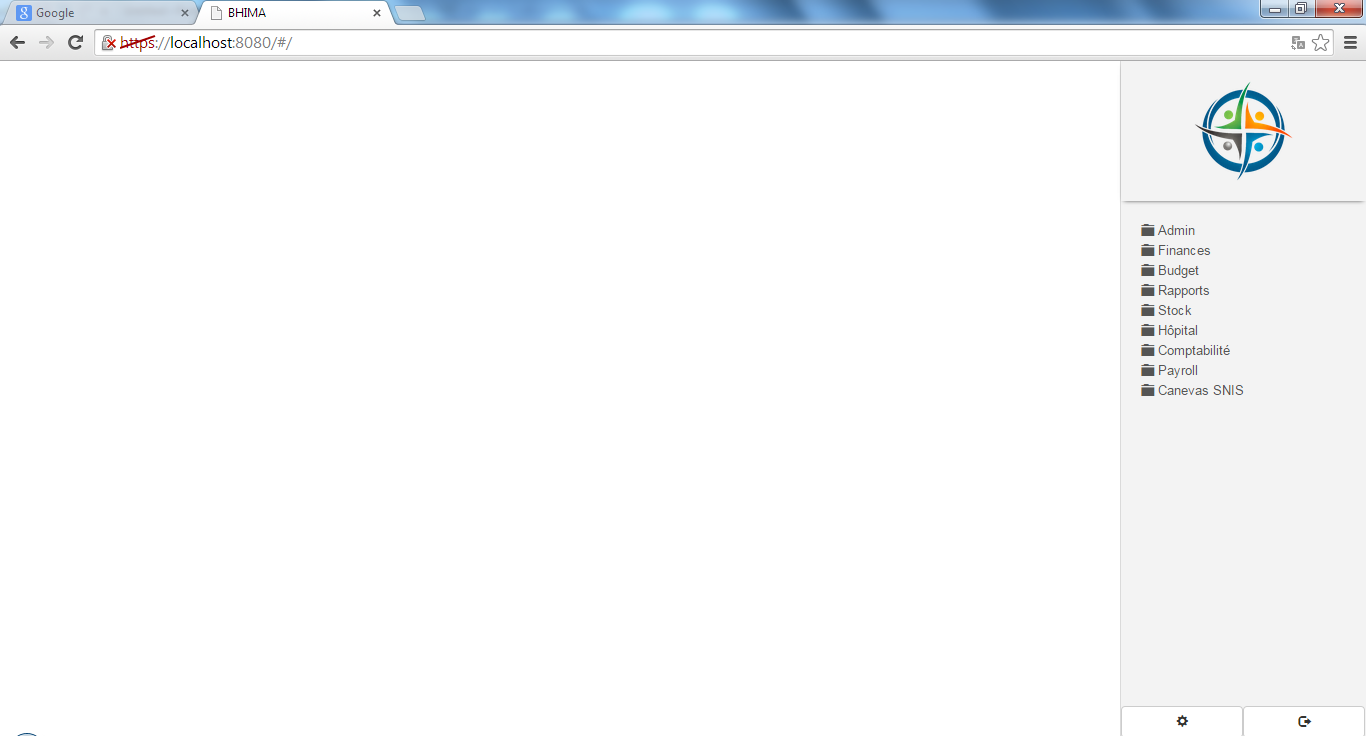
\includegraphics[width=10cm]{pic/mainInterface.png}
\end{center}
\caption{Interface principale de l'application}
\label{Interface principale de l'application}
\end{figure} 
Dans sa partie gauche de la figure ci-dessous on retrouve le logo IMA World Heath Ainsi que l'arborescence qui représente les modules du système auxquels l'utilisateur à accès. En dessous de l'arborescence figure deux boutons, le premier 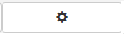
\includegraphics[scale=0.5]{pic/lang.png} permet de changer de langue et le second 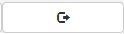
\includegraphics[scale=0.5]{pic/logout.png} permet de ce déconnecté du système.

\begin{figure}[h]
\begin{center}
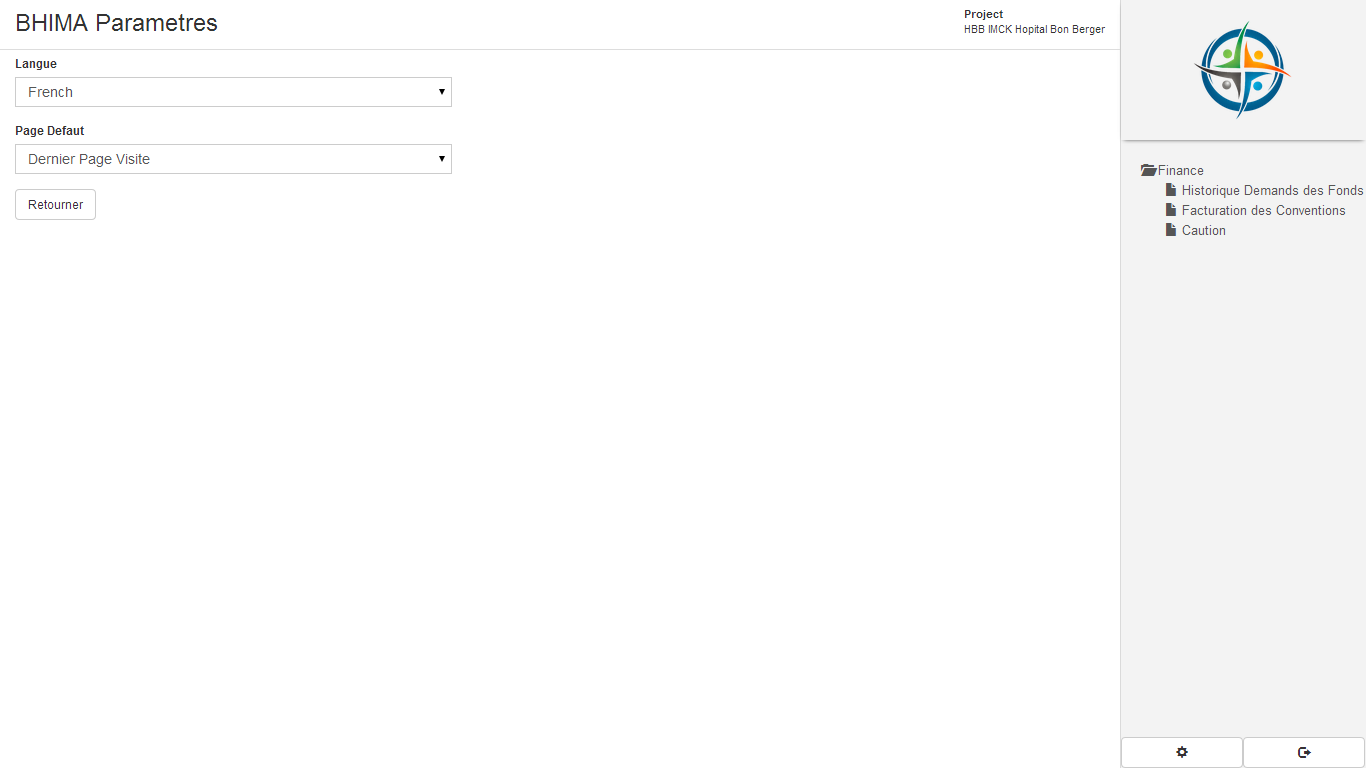
\includegraphics[width=10cm]{pic/changeLang.png}
\end{center}
\caption{Interface principale pour le changement de langue}
\label{Interface principale pour le changement de langue}
\end{figure} 

\section{Utilisation de l'arborescence de navigation}
L'arborescence de navigation contient les liens de chague module de l'application. Les modules sont regroupés en fonction de de leurs fonctionalités dans des dossiers tels que le dossier "Admin" affiché ci-dessous. Dans la première image, le dossier est fermé, en occultant tous les sous modules de ce module. Après le dossier est cliqué, une image d'un dossier ouvert montre que les contenus sont accessibles.

\begin{figure}[h]
\begin{center}
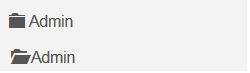
\includegraphics[width=4.5cm]{pic/folder_open_closed.png}
\end{center}
\caption{Etat d'un module ouvert et fermé}
\label{Etat d'un module ouvert et fermé}
\end{figure} 

Cliquant sur le dossier permet d'afficher la liste de sous modules sélectionné par l'utilisateur. Par exemple, ci-dessous, le dossier "Admin" est cliqué dans la premier illustration dans la séconde est ouverte tous ses sous modules.

\begin{figure}[h]
\begin{center}
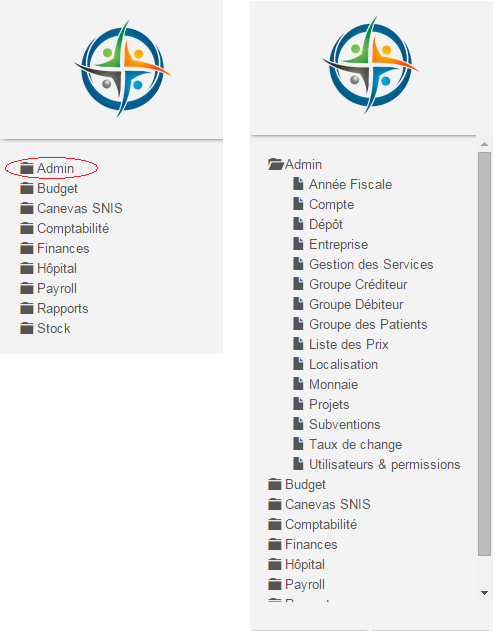
\includegraphics[width=8cm]{pic/open_folder.png}
\end{center}
\caption{Clique sur le dossier "admin" afin de pouvoir visualiser ses sous modules}
\label{Clique sur le dossier "admin" afin de pouvoir visualiser ses sous modules}
\end{figure} 


\newpage
\section{Les modules du système BHIMA}
Le système d'information BHIMA possède plusieurs modules qui sont représenté par l'arborescence ci-dessous.
\begin{figure}[h]
\begin{center}
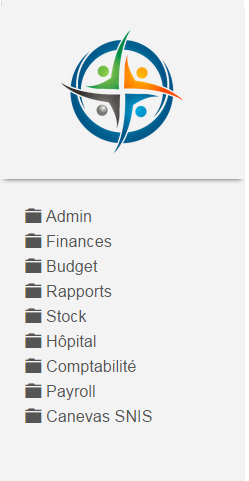
\includegraphics[width=4.5cm]{pic/arbo.png}
\end{center}
\caption{Arborescence du système}
\label{Arborescence du système}
Voici les différentes rubriques qui existent dans le système:
\end{figure} 
% Liste des modules
\begin{itemize}
\item Admin. %•
\item Budget
\item Canevas SNIS
\item Comptabilité
\item Finances
\item Hôpital
\item Payroll
\item Rapports
\item Stock
\end{itemize}


\newpage
%%%%%%%%%%%%%%%%%%%%%%%%%%%%%%%%%%%%%%%%%%%%%
%   MODULES DU SYSTEMES                     %
%%%%%%%%%%%%%%%%%%%%%%%%%%%%%%%%%%%%%%%%%%%%%

\newpage
\chapter{Stock}        
%////////////////////////////////////////////////%
Le module Stock est composé des sous modules qui permettent d'administrer le stock. La figure ci-dessous représente avec exactitude ce module avec ses différents sous éléments.

\begin{figure}[h]
\begin{center}
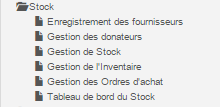
\includegraphics[width=6cm]{pic/StockManagement.png}
\end{center}
\caption{Arborescence du module Stock}
\label{Arborescence du module Stock}
\end{figure}



\newpage
\section{Gestion de stock}
Le sous module gestion de stock permet de faire plusieurs types opération relative à la gestion de stock, l'interface principale de ce module liste en fait les différents dépots qui sont configurer dans le système \textbf{Voir le module gestion de dépôt dans le répertoire Admin de l'arborescence de l'application}. voici l'apperçue de l'interface principale du sous module gestion de stock.

\begin{figure}[h]
\begin{center}
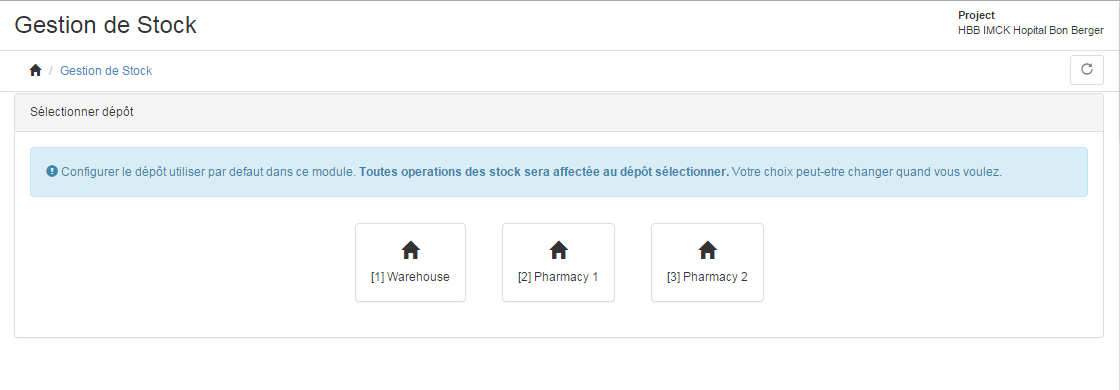
\includegraphics[width=12cm]{pic/MenuGestStock.png}
\end{center}
\caption{Apperçue de module gestion de stock}
\label{Apperçue de module gestion de stock}
\end{figure}

Dans la figure ci haute on a la possibilité de pouvoir choisir parmi les dépôts celui dont on voudrai administrer le stock, et une fois qu'on clique sur un dépôt, le menu d'administration de dépôts apparait à noter aussi que si l'on a sélectionné un dépôt, c'est ce dépôt qui sera utilisé à chaque fois qu'on accèdera à ce module et si l'on veut choisir un autre dépôt il suffit de cliquer sur le bouton 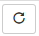
\includegraphics[scale=0.7]{pic/refresh.png} pour annuler la sélection qui a été faite.

Voici un apperçue du menu permettant de faire la gestion de dépôt.

\begin{figure}[h]
\begin{center}
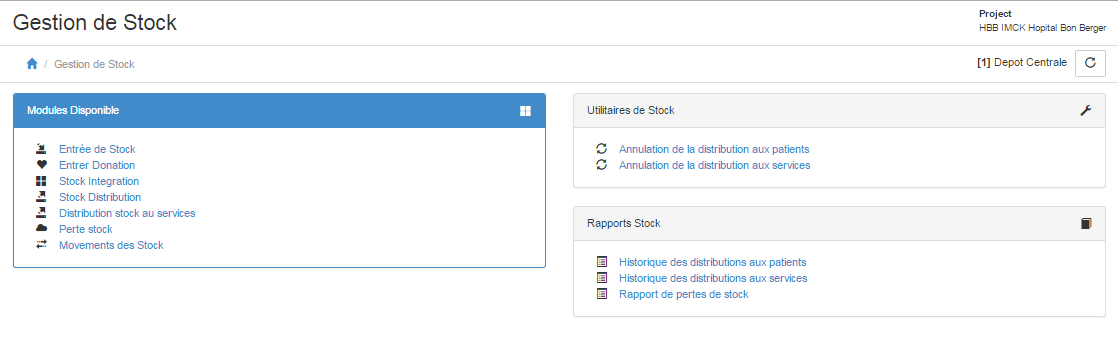
\includegraphics[width=12cm]{pic/MenuStock.png}
\end{center}
\caption{Menu permettant de faire la gestion de dépôt}
\label{Menu permettant de faire la gestion de dépôt}
\end{figure} 

Dans le coin supérieur gauche est écrite le nom du dépôt qui a été sélectionné ainsi que le bouton 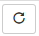
\includegraphics[scale=0.7]{pic/refresh.png} qui permet de revenir au menu principale du module gestion de stock pour permettre la sélection d'un nouveau dépôt.

Dans la partie qui se trouve au centre ont retrouve à gauche la liste des modules disponibles et à droite l'utilitaire du stock ainsi que le rapport de stock.


\subsection{Entrée de Stock}
le module entrée de stock permet d'approvisionné le stock dans un dépôt, cette opération est précedé d'une commande d'achat qui a était emise via le module \textbf{Gestion des commandes d'achat}. L'interface principale permettant de d'entrer le stock dispose d'une zone de saisie \textbf{Choisir une commande d'achat} qui permet de saisir la référence de la commande d'achat.

\begin{figure}[h]
\begin{center}
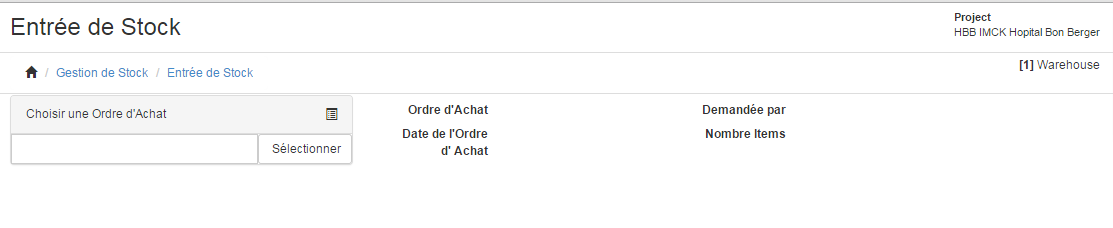
\includegraphics[width=12cm]{pic/EntreStock.png}
\end{center}
\caption{Interface principale du module entrée de stock}
\label{Interface principale du module entrée de stock}
\end{figure}

Une fois que la zone de saisie est renseignée, il suffit de cliquer sur le bouton  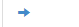
\includegraphics[scale=0.7]{pic/BlueArrow.png} pour que l'interface permettant d'approvisionner le stock puisse apparaitre comme le montre la figure ci après.

\begin{figure}[h]
\begin{center}
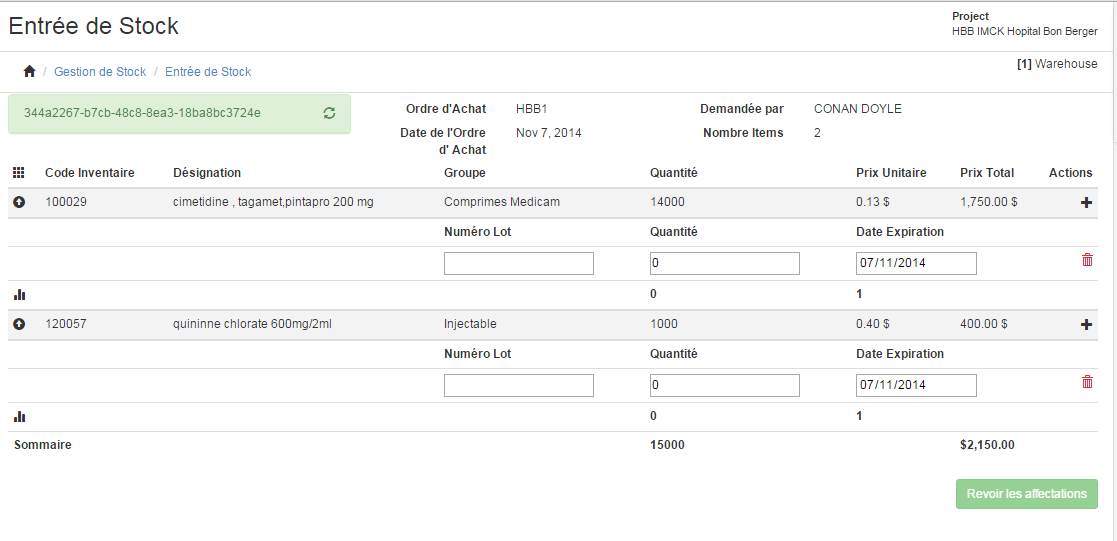
\includegraphics[width=14cm]{pic/EntreStockForm.png}
\end{center}
\caption{Apperçue du processus d'approvisionement de stock}
\label{Apperçue du processus d'approvisionement de stock}
\end{figure}

\newpage

Dans la partie supérieur on retrouver à gauche l'identifiant de la commande d'achat, et au milieu la référence de la commande d'achat la data dans laquelle la commande d'achat a été emise, le nom de la personne qui s'est chargé de l'achat, ainsi que le nombre des items concerné dans la commande d'achat.

Dans la partie médianne on retrouve un tableau listant les différents items de la commande d'achat, ce tableau possède plusieur entête dont: Le Code de l'inventaire, la désignation de l'item, le groupe dans lequel fait partie ce médicament, la quantité disponible, le prix de vente unitaire, le prix total ainsi que la zone action.

Pour chaque item on retrouve une zone permettant de spécifier le numéro de lot du fabriquant, la quantité à entreposer ainsi que la date d'expiration du produit comme le montre la figure ci après.

\begin{figure}[h]
\begin{center}
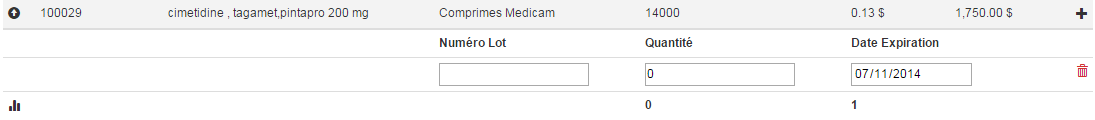
\includegraphics[width=12cm]{pic/illustrationStock.png}
\end{center}
\caption{Apperçue de la zone permettant la configuration d'un item}
\label{Apperçue de la zone permettant la configuration d'un item}
\end{figure}

Et si lors de l'opération de réapprovisionement d'un item, l'on disposait de deux lots de ce même article, le bouton 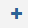
\includegraphics[scale=0.7]{pic/PlusGray.png} permet d'ajouter une ligne dans la zone rélative à la spécification du numéro de lot du fabriquant, la quantité etc...

\begin{figure}[h]
\begin{center}
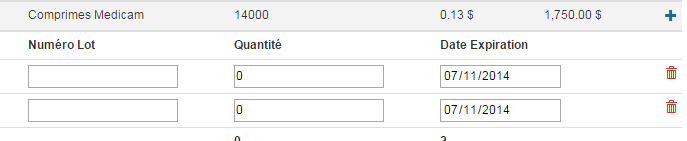
\includegraphics[width=12cm]{pic/ForAddPlus.png}
\end{center}
\caption{Apperçue du dispositif de configuration d'item qui dispose de plusieur lots}
\label{Apperçue du dispositif de configuration d'item qui dispose de plusieur lots}
\end{figure}

Et si l'on desire supprimer une ligne dans ce dispotif, il suffit de cliquer sur le bouton 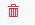
\includegraphics[scale=0.7]{pic/DeleteWRed.png} qui permet de supprimer une ligne dans la configuration.

Et lors de la saisie des données concernant un item qui dispose de plusieur lots ou non, la quantité total doit toujours être égale à celui se trouvant dans la commande d'achat si non le processus d'approvisionement sera impossible.

La figure ci après est une illustration d'un cas de figure ou l'on procede par l'approvisionement de deux items dont le premier dispose de deux lots.

\begin{figure}[h]
\begin{center}
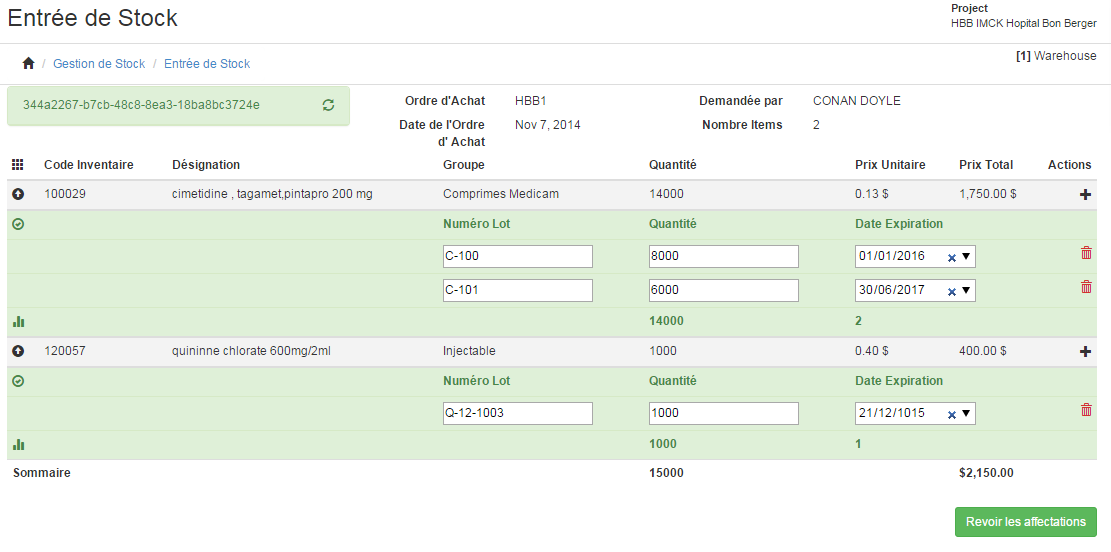
\includegraphics[width=12cm]{pic/AppStockOK.png}
\end{center}
\caption{Apperçue de l'illustration de l'approvisionement}
\label{Apperçue de l'illustration de l'approvisionement}
\end{figure}

Une fois que les éléments rélative à l'approvisionement sont renseignés, il suffit de cliquer sur le bouton 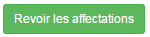
\includegraphics[scale=0.7]{pic/RevAffectation.png} qui permet d"afficher l'interface permettant de revoir le processus d'approvisionnement de stock et si il n' y a pas d'erreur il suffit de cliquer sur le bouton \textbf{Faire entrer les stock} pour valider le réapprovisionement du stock dans le système.

\begin{figure}[h]
\begin{center}
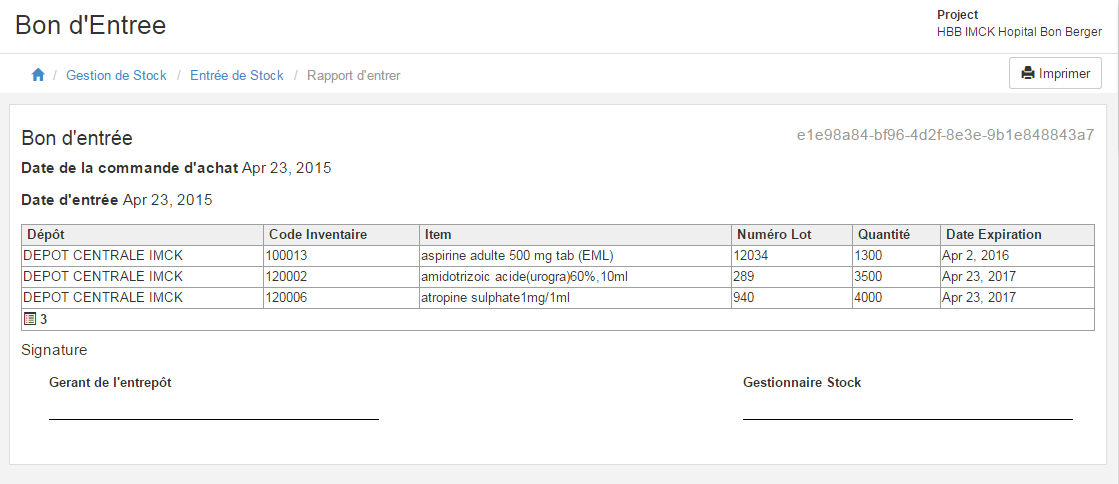
\includegraphics[width=12cm]{pic/EntreStockEnter.png}
\end{center}
\caption{Apperçue du bon d'entrée en stock}
\label{Apperçue du bon d'entrée en stock}
\end{figure}

\subsection{Stock Distribution}
le module stock distribution permet la distribution des produits à un patient, pour utiliser ce module le patient devrait premièrement être facturé et en suite passé par la caisse pour le règlement de la facture, mais pour ceux qui sont conventionnés, pris en charges et même ceux qui sont couvertes par une caution peuvent directement passer à l'officine pour pouvoir obtenir les produits pharmaceutiques.

L'interface principale de ce module dispose d'une zone qui permet de rechercher le patient soit par son ID Débiteur ou bien directement par son nom. La figure ci après représente l'interface principale de ce module.

\begin{figure}[h]
\begin{center}
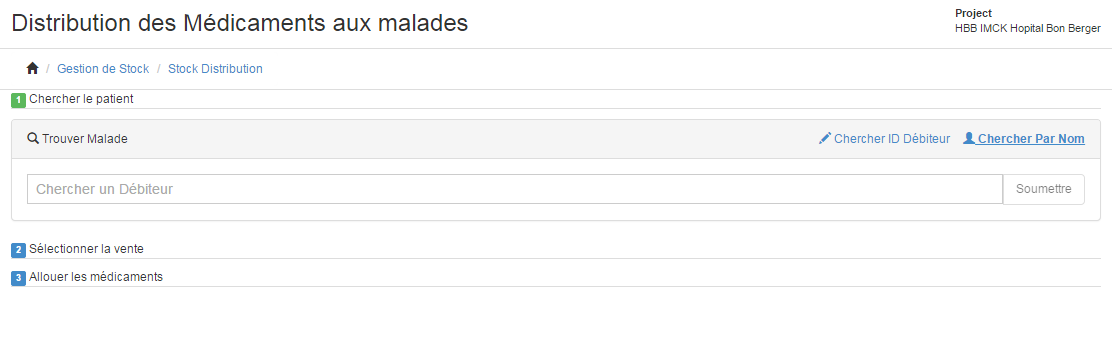
\includegraphics[width=12cm]{pic/DistrMediMalade.png}
\end{center}
\caption{Apperçue de l'interface principale de la distribution des stocks}
\label{Apperçue de l'interface principale de la distribution des stocks}
\end{figure}

Une fois que le patient a été trouvé, il suffit de cliquer sur le bouton \textbf{Soumettre} pour savoir si le patient dispose des factures liée à la livraison des produits pharmacautiques, s'il n'en disposait pas le message suivant apparaitra à l'écran comme le montre la figure suivante.

\begin{figure}[h]
\begin{center}
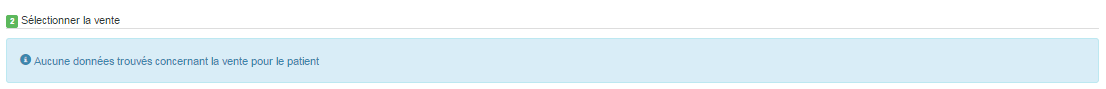
\includegraphics[width=14cm]{pic/NoSaleFound.png}
\end{center}
\caption{Apperçue du message montrant que le patient n'est lié à aucune vente}
\label{Apperçue du message montrant que le patient n'est lié à aucune vente}
\end{figure}

Et si le patient est liée à des ventes qui ne concernent pas les produits pharmaceutiques ou bien qui concernent des produits qui ne sont pas en stock le message suivant apparaitra à l'ecran.

\begin{figure}[h]
\begin{center}
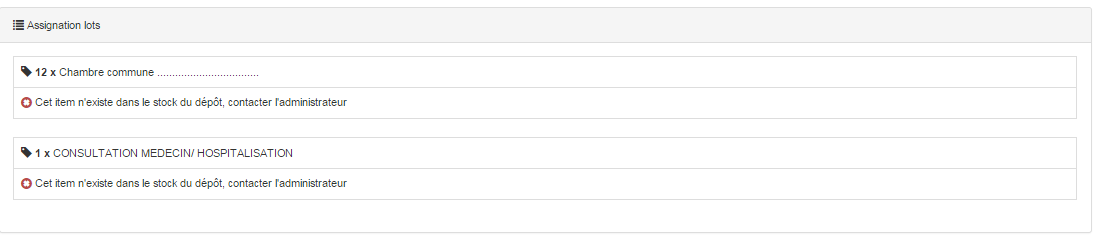
\includegraphics[width=14cm]{pic/NotInStock.png}
\end{center}
\caption{Apperçue du message concernant les produits qui ne sont pas en stock}
\label{Apperçue du message concernant les produits qui ne sont pas en stock}
\end{figure}

Dans le cas ou le patient est lié à des produits pharceutiques mais n'est pas encore passé par la facturation, le système le signalera aussi tôt, la figure suivante donne l'illustration d'un cas de vente impayée.

\begin{figure}[h]
\begin{center}
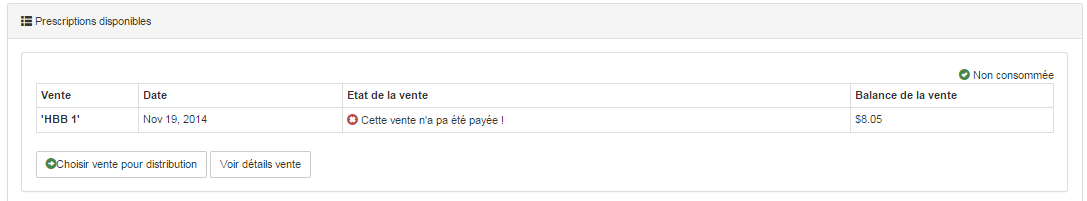
\includegraphics[width=14cm]{pic/NotPaid.png}
\end{center}
\caption{Apperçue du message concernant les ventes impayés}
\label{Apperçue du message concernant les ventes impayés}
\end{figure}

Dans le cas d'une facture qui a été totalement payée, l'interface se présente de la manière suivante.

\begin{figure}[h]
\begin{center}
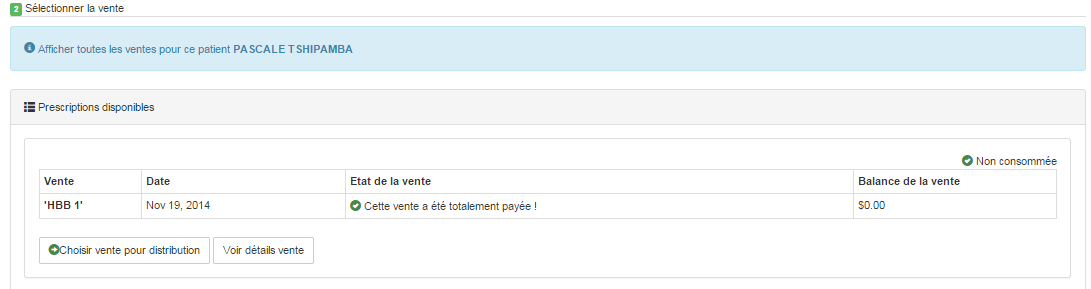
\includegraphics[width=14cm]{pic/TotalPaid.png}
\end{center}
\caption{Apperçue de l'interface pour les factures totalement payée}
\label{Apperçue de l'interface pour les factures totalement payée}
\end{figure}

\newpage

Sur cette interface on retrouve la date de la vente, l'état de la vente par lequel on sait que la facture a été payé, la balance de vente et en dessous de cette zone, existe deux boutons le premier permet de \textbf{Choisir cette vente pour une distribution} et le second permet de \textbf{Voir le detail de la vente}. 

Pour pouvoir executer une distribution il faudrait cliquer sur le bouton 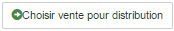
\includegraphics[scale=0.7]{pic/ChoisirDistr.png} pour être rediriger vers l'interface permettant de faire la distribution.

L'interface permettant de faire la distribution des médicaments se présente de la manière suivante.

\begin{figure}[h]
\begin{center}
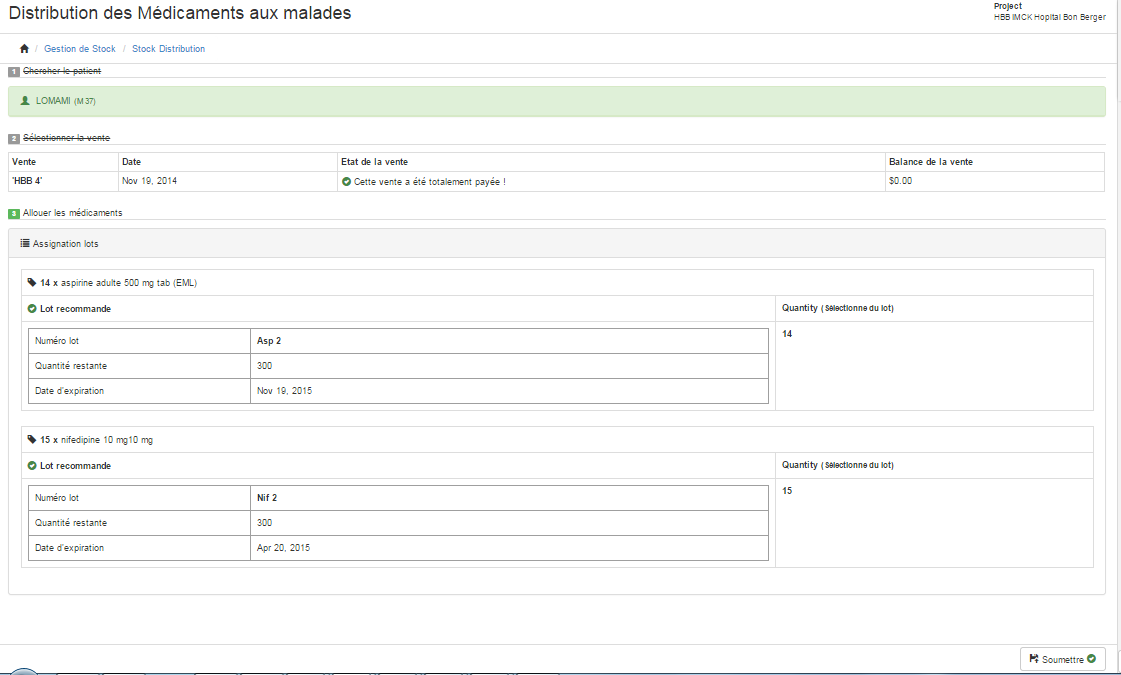
\includegraphics[width=14cm]{pic/DistrMedPatient.png}
\end{center}
\caption{Apperçue de l'interface permettant la distribution des médicaments}
\label{Apperçue de l'interface permettant la distribution des médicaments}
\end{figure}

Dans l'entête de cette interface on retrouve l'identité du patient, la date, l'état de la vente, la balance de la vente, dans la zone 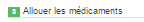
\includegraphics[scale=0.7]{pic/AllocateDrug.png} se trouve toutes les informations concernant les produits à distribué, le système propose automatiquement le lot qu'il faudrait utilisait pour la livraison, la quantité restante ainsi que la quantité à livrer.

Pour confirmer la livraison des produits, il suffit de cliquer sur le bouton 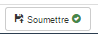
\includegraphics[scale=0.7]{pic/SoumettreDistribution.png}.

Le système BHIMA detecte la péremption des produits pharmaceutiques lors de l'opération de livraison des produits pharmaceutiques en affichant des messages d'alerte à l'écran de l'ordinateur comme le montre la figure suivante.

\begin{figure}[h]
\begin{center}
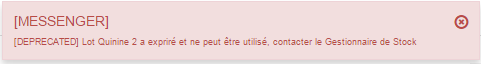
\includegraphics[width=10cm]{pic/expirationDrug.png}
\end{center}
\caption{Apperçue du message prévenant la péremption des médicaments}
\label{Apperçue du message prévenant la péremption des médicaments}
\end{figure}

Le système avertit aussi lorsque la quantité en stock ne permet pas de couvrir la vente en affichant le message d'alerte suivante.

\begin{figure}[h]
\begin{center}
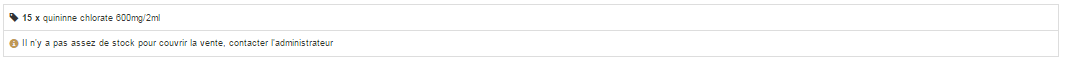
\includegraphics[width=14cm]{pic/InsuffStock.png}
\end{center}
\caption{Apperçue du message prévenant l'insuffisance du stock}
\label{Apperçue du message prévenant l'insuffisance du stock}
\end{figure}

Le système donne aussi des orientations par rapport à la manière de livrer les produits dans le cas où pour un produits ont dispose simultanement de deux lots en stock.  

\begin{figure}[h]
\begin{center}
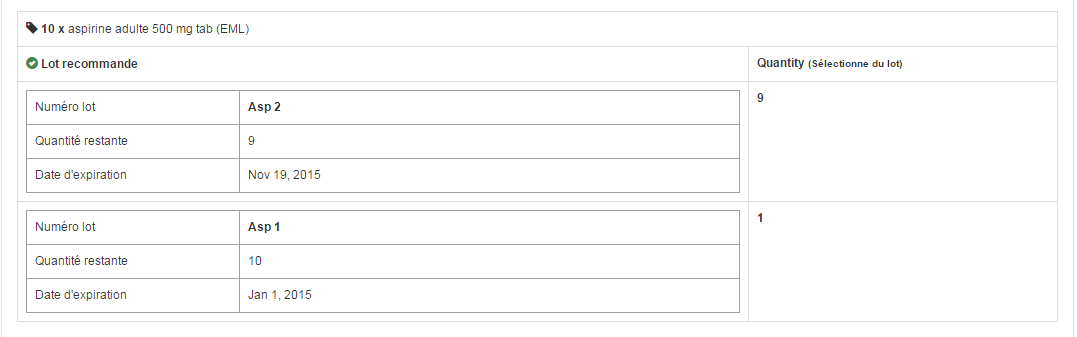
\includegraphics[width=14cm]{pic/AstuceDistribution.png}
\end{center}
\caption{Apperçue de l'interface prevenant l'orientation de la distribution}
\label{Apperçue de l'interface prevenant l'orientation de la distribution}
\end{figure}

Dans l'image ci haut on peut se rendre compte la quantité à livrer du produit est supérieur au premier lot proposé et le système propose automatiquement un autre lot et avec la quantité à utiliser pour effectué la livraison.

\newpage
\subsection{Distribution stock aux services}
Le module distribution stock au services permet de repartir les médicaments dans le service existant au sein de l'hôpital.

L'interface principale de ce module se présente de la manière suivante. 

\begin{figure}[h]
\begin{center}
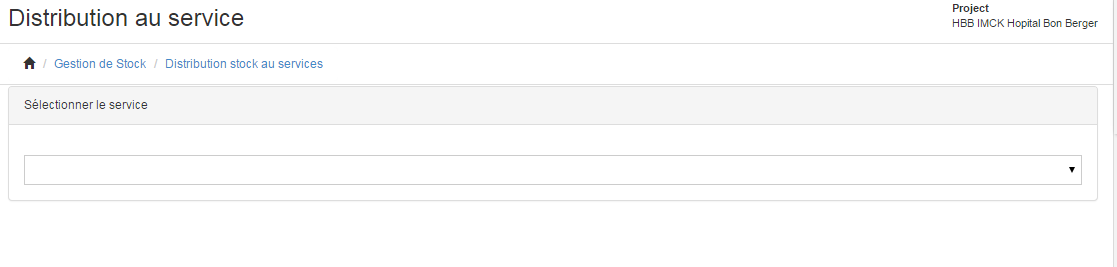
\includegraphics[width=14cm]{pic/DistService.png}
\end{center}
\caption{Interface principale de la distribution de stock aux services}
\label{Interface principale de la distribution de stock aux services}
\end{figure}


Dans cette interface on retrouve une zone permettant de rechercher les services existants dans l'organisations, une fois qu'on a choisi l'un d'entre eux, l'interface permettant de faire la distribution apparait. Dans cette interface on retrouve les informations sommaires sur les services qui a été choisi, et precise à l'utilisateur sur le dépôt qui est prise en compte pour la distribution. Voici un apperçue de cette interface.

\begin{figure}[h]
\begin{center}
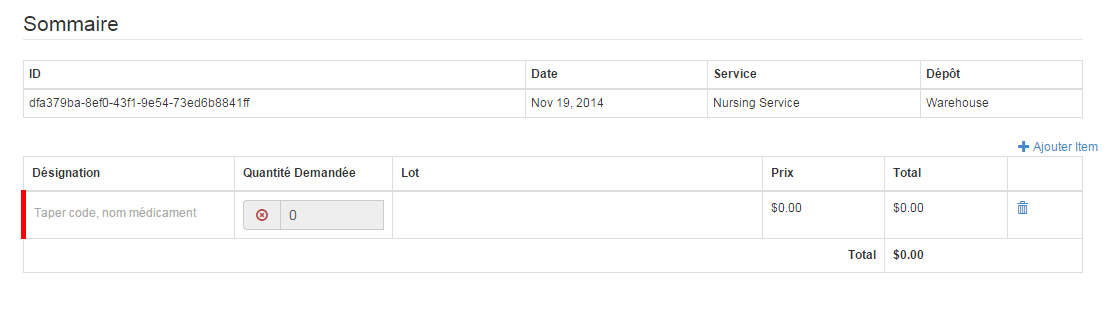
\includegraphics[width=14cm]{pic/FormulaireDistrService.png}
\end{center}
\caption{Formulaire de la distribution de stock aux services}
\label{Formulaire de la distribution de stock aux services}
\end{figure}
\newpage
Pour faire la distribution des médicaments il faut premièrement commencer rechercher les produits dans la zone 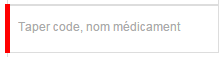
\includegraphics[scale=0.7]{pic/RecherMedicament.png} cette zone fonctionne comme un filtre, et une fois qu'un produit est choisi, il suffit de preciser la quantité demandée pour connaitre si le produit est en stock ou si la quantité demandée peut être servi, le bouton 
\includegraphics[scale=0.7]{pic/RecycleBlue.png} qui permet de supprimer une ligne dans la configuration. 

\begin{figure}[h]
\begin{center}
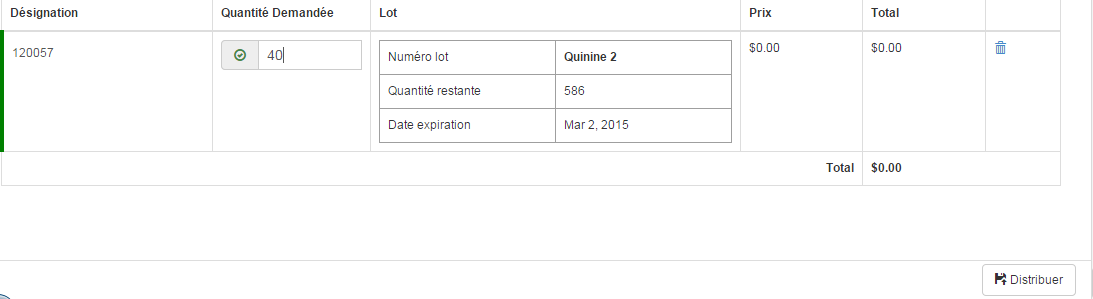
\includegraphics[width=14cm]{pic/procDistService.png}
\end{center}
\caption{Apperçue du processus de distribution de stock aux services}
\label{Apperçue du processus de distribution de stock aux services}
\end{figure}

Une fois que la quantité est renseigné, il suffit de cliquer sur le bouton \textbf{Distribuer} pour pouvoir confirmer la distribution.

Si l'on desire faire la distribution des plusieurs services en même temps il est possible de le faire juste en cliquant sur le bouton 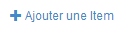
\includegraphics[scale=0.7]{pic/AjouterItem.png} pour pouvoir ajouter une nouvelle ligne.

Le module distribution ne concerne que les produits qui sont en stock, et si la quantité demandé est supérieur à celle qui est en stock cette opération ne pourra pas s'executer mais pour les produits qui sont en stock avec plusieurs lots le système permet d'orienter sur la façon dont pourait se faire la distribution en précisant la repartition par lots.

\newpage
\subsection{Perte Stock}
Le module perte stock permet de faire plusieurs opérations à la fois:

\begin{itemize}
\item enregistrer les produits qui sont expirés
\item enregistrer les produits qui sont volés ou bien perdus
\item enregister les produits qui sont habimés ou bien qui sont devenus impropres à la consommation
\end{itemize}

l'interface principale de ce module se présente de la manière suivante.

\begin{figure}[h]
\begin{center}
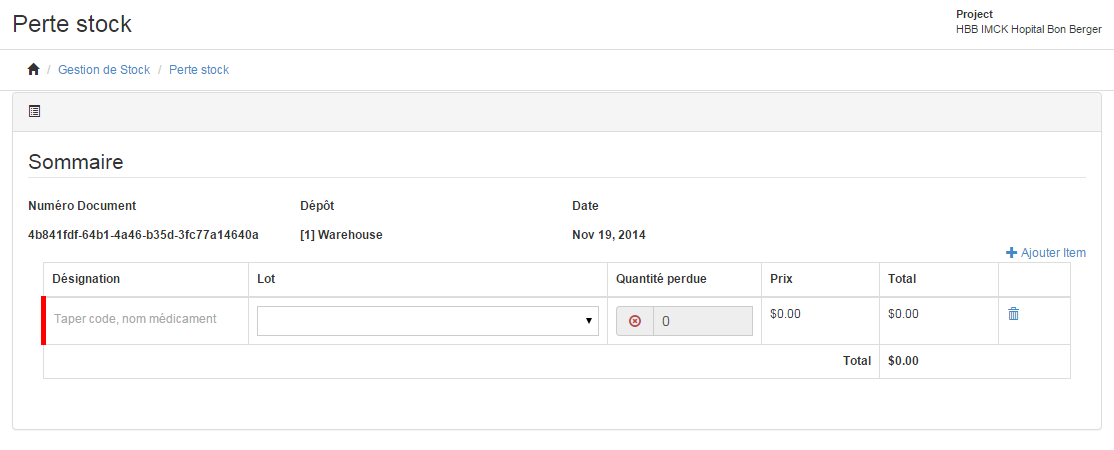
\includegraphics[width=14cm]{pic/PerteStock.png}
\end{center}
\caption{Interface principale du module perte de stock }
\label{Interface principale du module perte de stock }
\end{figure}


Dans cette interface on retrouve la référence du document, le dépôt concerné par la perte ainsi que la date. en dessous de cette zone on retrouve le bouton 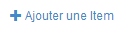
\includegraphics[scale=0.7]{pic/AjouterItem.png} qui permet d'ajouter une ligne dans l'interface permettant de sélectionner les produits qui sont concernés par la perte, le bouton 
\includegraphics[scale=0.7]{pic/RecycleBlue.png} qui permet de supprimer une ligne dans la configuration.


Pour selectionner un produit il faut premièrement commencer rechercher les produits dans la zone 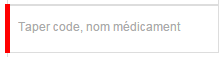
\includegraphics[scale=0.7]{pic/RecherMedicament.png} cette zone fonctionne comme un filtre, et une fois qu'un produit est choisi, il suffit de preciser le lot concernet par la perte ainsi que la quantité. pour confirmer la perte il faudrait cliquer sur le bouton 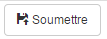
\includegraphics[scale=0.7]{pic/SubmitSave.png}.

La figure suivante illustre un cas de figure d'opération de perte de stock concerné par deux produits

\begin{figure}[h]
\begin{center}
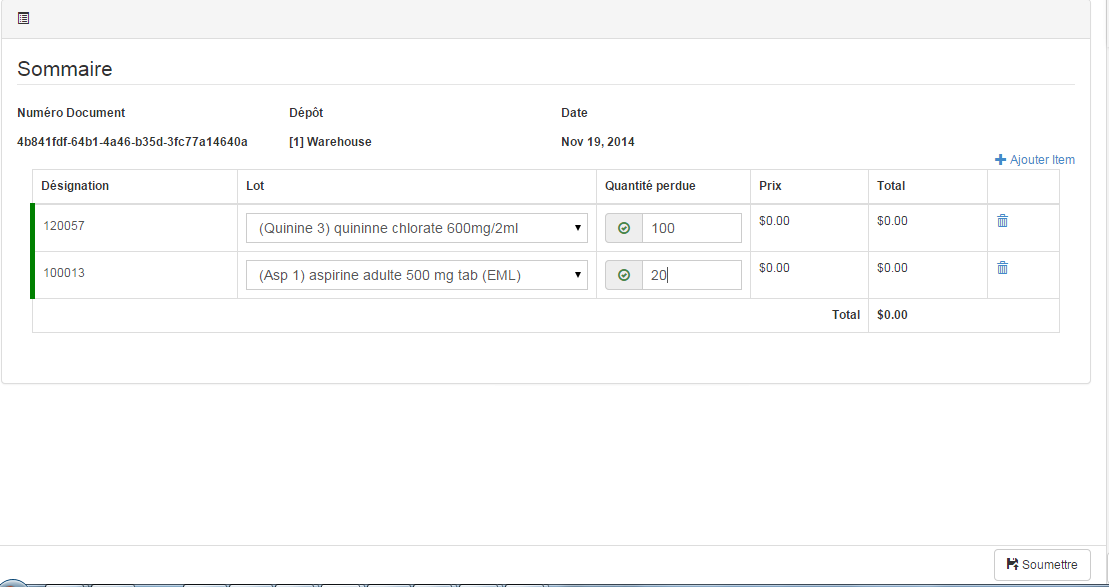
\includegraphics[width=14cm]{pic/PerteStockForm.png}
\end{center}
\caption{Apperçue de l'illustration de perte de stock}
\label{Apperçue de l'illustration de perte de stock}
\end{figure}

\newpage
\subsection{Mouvements des stock}
Le module mouvements des stock permet d'éffectuer les mouvements de stock entre deux dépôt pour ce son interface permet premièrement de sélectionnet le dépôt source et le dépôt destination. Voici l'interface principale de ce module.

\begin{figure}[h]
\begin{center}
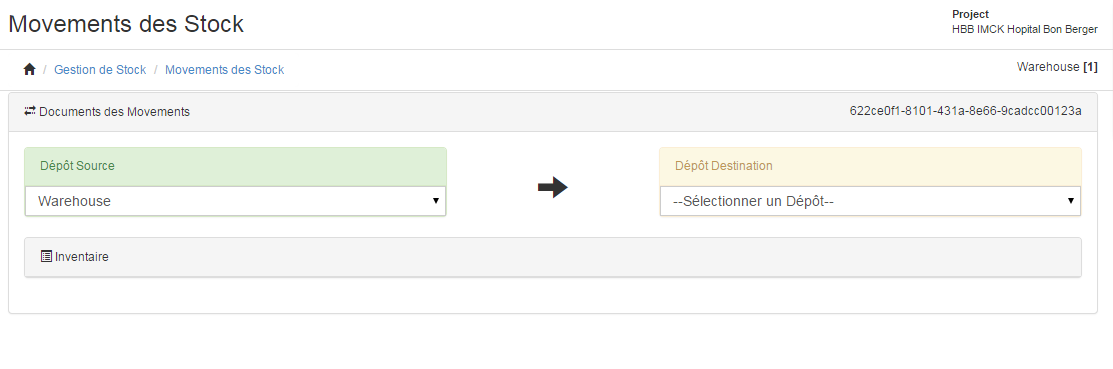
\includegraphics[width=14cm]{pic/MouvStock.png}
\end{center}
\caption{Interface principale du modules mouvements des stock}
\label{Interface principale du modules mouvements des stock}
\end{figure}

Après avoir designé les deux dépôts faisant parti du transfert, une nouvelle zone apparait, cette zone permet de preciser les produits à partir de leur numéro de lot qui font partie de l'opération mouvement de stock ainsi que la quantité à transferer. 
Voici le formulaire qui permet de faire l'opération de transfert.

\begin{figure}[h]
\begin{center}
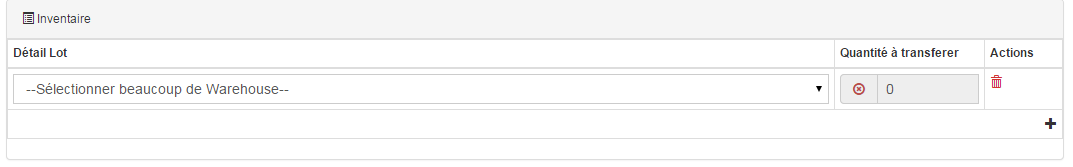
\includegraphics[width=14cm]{pic/SelectProduit.png}
\end{center}
\caption{Interface principale permettant de sélectionner les produits}
\label{Interface principale permettant de sélectionner les produits}
\end{figure}

\newpage

Si l'on sélectionne un produit à partir de son numéro de lot dans liste toutes les informations concernant les produits apparaisent à l'écran. Pour finaliser l'opération de mouvement de stock, il est necessaire de renseigner la quantité à transferer et cette quantité doit ne doit pas être supérieur à la quantié existante. Pour finaliser l'opération de transfert il suffit de cliquer sur le bouton \textbf{Soumettre} pour valider le transfert.

Si l'on desire ajouter une autre ligne pour le transfert des produits il suffit de cliquer sur le bouton \includegraphics[scale=0.7]{pic/plusBlack.png}. 

Voici un apperçue d'une interface de mouvement de stock concernant deux produits pharmaceutiques.

\begin{figure}[h]
\begin{center}
\includegraphics[width=14cm]{pic/DocMovTransfert.png}
\end{center}
\caption{Interface principale permettant de sélectionner les produits}
\label{Interface principale permettant de sélectionner les produits}
\end{figure}

\newpage
\subsection{Entrer donation}
Le module entrer donantion permet de faire la Gestion de Dons en médicaments ou bien en produits pharmaceutiques, l'interface principale du module se présente de la manière.

\begin{figure}[h]
\begin{center}
\includegraphics[width=14cm]{pic/GestionDon.png}
\end{center}
\caption{Interface principale du module Gestion de dons}
\label{Interface principale du module Gestion de dons}
\end{figure}

Dans la partie gauche de la figure ci-haute on retrouve une zone permettant la configuration de donation en précisant la date, le nom du donateur  ainsi que le responsable de l'enregistrement de dons en stock. Une fois que ses éléments sont designés, la zone qui se trouve à gauche permet d'enregistrer les produits qui font partie de la donation.

Dans l'entête de cette zone on retrouve le nom du donateur ainsi que le nom de la personne qui effectue l'enregistrement du don. En dessous de l'entête se trouve la zone permettant de rechercher les produits pharmaceutiques, de spécifier la quantité et en ceux qui concerne le don généralement le prix d'achat est nulle. le bouton \includegraphics[scale=0.7]{pic/AjArticleGreen.png} permet d'ajouter une ligne dans la configuration de dons. et une fois qu'on a fini avec l'enregistremet des produits faisant partie du don, il suffit de cliquer sur le bouton \includegraphics[scale=0.7]{pic/EnregistrLots.png} pour spécifier la repartition des chaques produits par rapport aux numéros de lots.

L'interface permettant de faire la repartion par lots se présente de la manière suivante.

\begin{figure}[h]
\begin{center}
\includegraphics[width=14cm]{pic/LotByDon.png}
\end{center}
\caption{Apperçue de l'interface permettant de faire la repartition d'un don par lot}
\label{Apperçue de l'interface permettant de faire la repartition d'un don par lot}
\end{figure}

Dans la partie médianne on retrouve un tableau listant les différents items de la donation, ce tableau possède plusieur entête dont: Le Code de l'inventaire, la désignation de l'item,  la quantité disponible, le prix de vente unitaire, le prix total ainsi que la zone action.

Pour chaque item on retrouve une zone permettant de spécifier le numéro de lot du fabriquant, la quantité à entreposer ainsi que la date d'expiration du produit comme le montre la figure ci après et si lors de l'opération d'enregistrement d'un item, l'on disposait de deux lots de ce même article, le bouton \includegraphics[scale=0.7]{pic/PlusGray.png} permet d'ajouter une ligne dans la zone rélative à la spécification du numéro de lot du fabriquant, la quantité etc...

\begin{figure}[h]
\begin{center}
\includegraphics[width=12cm]{pic/ForAddPlus.png}
\end{center}
\caption{Apperçue du dispositif de configuration d'item qui dispose de plusieur lots}
\label{Apperçue du dispositif de configuration d'item qui dispose de plusieur lots}
\end{figure}

Et si l'on desire supprimer une ligne dans ce dispotif, il suffit de cliquer sur le bouton \includegraphics[scale=0.7]{pic/DeleteWRed.png} qui permet de supprimer une ligne dans la configuration.

Et lors de la saisie des données concernant un item qui dispose de plusieur lots ou non, la quantité total doit toujours être égale à celui se trouvant dans la commande d'achat si non le processus d'approvisionement sera impossible.

La figure ci après est une illustration d'un cas de figure ou l'on procede par l'approvisionement de deux items dont le premier dispose de deux lots.

\begin{figure}[h]
\begin{center}
\includegraphics[width=12cm]{pic/AppStockOK.png}
\end{center}
\caption{Apperçue de l'illustration de l'approvisionement}
\label{Apperçue de l'illustration de l'approvisionement}
\end{figure}
\newpage

Une fois que les éléments rélative à l'approvisionement sont renseignés, il suffit de cliquer sur le bouton \includegraphics[scale=0.7]{pic/RevAffectation.png} qui permet d"afficher l'interface permettant de revoir le processus d'approvisionnement de stock et si il n' y a pas d'erreur il suffit de cliquer sur le bouton \textbf{Faire entrer les stock} pour valider le réapprovisionement du stock dans le système.

\begin{figure}[h]
\begin{center}
\includegraphics[width=12cm]{pic/BonEntryDonation.png}
\end{center}
\caption{Apperçue du bon d'entrée d'une donation}
\label{Apperçue du bon d'entrée d'une donation}
\end{figure}

\newpage
\section{Tableau de bord du Stock}
Le tableau de bord du stock est une interface permettant de visualiser plus informations rélative à la gestion des stock. L'interface principale de ce module se présente de la manière suivante.

\begin{figure}[h]
\begin{center}
\includegraphics[width=12cm]{pic/TaBordStock.png}
\end{center}
\caption{Interface principale du Tableau de bord du stock}
\label{Interface principale du Tableau de bord du stock}
\end{figure} 

Le tableau de bord de stock permet de renseigner sur les 10 meilleurs produits les plus consommés, il s'agit pour cela des toutes les distributions des produits au près des patients et au près des services. 

le tableau de bord permet aussi de renseigner sur l'état des commandes qui ont eu lieu en renseignant sur:
\begin{itemize}
\item les nombres des commandes d'achat qui ont était effectué mais qui n'ont pas encore était payé (en attente de paiement);
\item les nombres des commandes d'achat pour les quels la caisse principale a effectué les paiements (payés);
\item les nombres des commandes pour lesquels il n' y a pas encore eu d'entrée en stock (en attente de reception);
\item les nombres des commandes pour lesquels il n' y a eu effectivement entrée en stock (reçues);
\end{itemize}

Le tableau de bord donne aussi des informations du stock par produits, on peut ainsi connaitre le nombre des produits qui sont en ruptire des stock, le nombres des produits pour lesquels la quantité existante est en dessous de la quantité minimal optimal en stock , ceux qui ont une quantité supérieur à la quantité maximal optimum en stock mais aussi le nombre de ceux dont la quantité en stock est optimale.

Le tableau de bord donne aussi un apperçue sur la péremption des médicaments en indiquant les nombres des produits encore en stock et qui ont expirés, ainsi que plusieurs échéances d'expiration des médicaments et les nombres des produits rélative en chacun d'entre eux.

Le tableau de bord renseigne aussi sur les produits qui ont étaient acquis grâce à des oeuvres des charités ou bien de dons, en listant les 10 derniers qui ont eu lieu dans un tableau qui permet de connaitre le nom du donateur ainsi que la date de la donation.

Le tableau de bord permet de sa rubrique rapports d'avoir un apperçue sur la situation glôbale en stock ainsi que sur la quantité des produits à risque de péremption.




\newpage
\chapter{Le module Rapports}        
%////////////////////////////////////////////////%
Le module rapports permet de pouvoir visualiser plusieurs types des rapports résultants du fonctionnements du système, La figure ci-dessous représente avec exactitude ce module avec les différents sous éléments.

\begin{figure}[h]
\begin{center}
\includegraphics[width=4cm]{pic/ArboReport.png}
\end{center}
\caption{Arborescence du module Rapports}
\label{Arborescence du module Rapports}
\end{figure}


\newpage
\section{Rapport des commandes d'achat}
Le rapport de confirmation des commandes d'achat permet de visualiser l'historique de confirmation de commande d'achatdans le système. L'interface principale permettant de voire le rapport d'enregistrement des patients se présente de la manière suivante. 

\begin{figure}[h]
\begin{center}
\includegraphics[width=10cm]{pic/RapConfPO.png}
\end{center}
\caption{Aperçue de l'interface principale du rapport de confirmation des commandes d'achat}
\label{Aperçue de l'interface principale du rapport de confirmation des commandes d'achat}
\end{figure}


La première zone permet de sélectionner le type de commande pour lequel on voudriai visualiser le rapport d'enregistrement, il y'a aussi une zone qui permet de spécifier l'écheance temporelle  ou bien spécifier directement la date du début et celle de la fin de la recherche. 

Le bouton générer permet l'affichage du tableau du rapport de confirmation de commande d'achat. L'interface permettant de visualier le rapport se présente de la manière suivante. Au dessus on retrouve deux boutons. le prémier 
\includegraphics[scale=0.7]{pic/Print.png} permet d'imprimer le rapport et le second \includegraphics[scale=0.7]{pic/refresh.png} permet de faire une nouvelle recherche.

\begin{figure}[h]
\begin{center}
\includegraphics[width=12cm]{pic/RapportCommAchat.png}
\end{center}
\caption{Aperçue du résultat du rapport de confirmation des commandes d'achat}
\label{Aperçue du résultat du rapport de confirmation des commandes d'achat}
\end{figure}

\newpage
\section{Confirmation des donations}
Le rapport de Confirmation des donations permet de visualiser l'historique de confirmation Confirmation des donations dans le système. L'interface principale permettant de voire le rapport d'enregistrement des patients se présente de la manière suivante. 

\begin{figure}[h]
\begin{center}
\includegraphics[width=10cm]{pic/RapConfPO.png}
\end{center}
\caption{Aperçue de l'interface principale du rapport de Confirmation des donations}
\label{Aperçue de l'interface principale du rapport de Confirmation des donations}
\end{figure}


La première zone permet de spécifier l'écheance temporelle  ou bien spécifier directement la date du début et celle de la fin de la recherche. 

Le bouton générer permet l'affichage du tableau du rapport de confirmation Confirmation des donations. L'interface permettant de visualier le rapport se présente de la manière suivante. Au dessus on retrouve deux boutons. le prémier 
\includegraphics[scale=0.7]{pic/Print.png} permet d'imprimer le rapport et le second \includegraphics[scale=0.7]{pic/refresh.png} permet de faire une nouvelle recherche.

\begin{figure}[h]
\begin{center}
\includegraphics[width=12cm]{pic/RapConfDon.png}
\end{center}
\caption{Aperçue du résultat du rapport de confirmation des donations}
\label{Aperçue du résultat du rapport de confirmation des donations}
\end{figure}

\newpage
\section{Consommation journalière}
Le module consommation journalière permet de lister la consommation journalière des produits pharmaceutiques dans le système.
son interface principale se présente de la manière suivante.

\begin{figure}[h]
\begin{center}
\includegraphics[width=14cm]{pic/ConsJour.png}
\end{center}
\caption{Interface principale du module consommation journalière}
\label{Interface principale du module consommation journalière}
\end{figure}

La figure ci haute est une illustration l'interface principale de la consommation journalière, cette interface permet de sélectionner la plage de temps pour laquelle on voudrait visualiser le rapport de la consommation. 

Le bouton générer permet l'affichage du tableau du rapport de la consommation journalière.
L'interface permettant de visualier le rapport se présente de la manière suivante. Au dessus on retrouve deux boutons. le prémier 
\includegraphics[scale=0.7]{pic/Print.png} permet d'imprimer le rapport et le second \includegraphics[scale=0.7]{pic/refresh.png} permet de faire une nouvelle recherche.

Le tableau du rapport de la consommation possède trois entête Code, Médicaments et Quantité total. Le code du médicament est un lien hypertexte qui permet une rédirection vers un autre rapport qui détaille la consommation effective d'un médicament par jour. 

\begin{figure}[h]
\begin{center}
\includegraphics[width=14cm]{pic/ConsoJournProd.png}
\end{center}
\caption{Apperçue du Consommation journalière}
\label{Apperçue du Consommation journalière}
\end{figure}


La figure ci-après donne un apperçue du rapport de consommation journalière d'un produit par jour.

\begin{figure}[h]
\begin{center}
\includegraphics[width=14cm]{pic/ConsoDetJourn.png}
\end{center}
\caption{Apperçue de la consommation détaillée d'un produit}
\label{Apperçue de la consommation détaillée d'un produit}
\end{figure}


\newpage
\section{Historique des distributions aux patients}
Le module historique des distributions aux patients, permet de visualiser la consommation en produits pharmaceutiques des patients dans une plage de temps données.

L'interface principale de ce module se présente de la manière suivante

\begin{figure}[h]
\begin{center}
\includegraphics[width=14cm]{pic/HistDistrPatient.png}
\end{center}
\caption{Interface principale du module Historique des distributions aux patients}
\label{Interface principale du module Historique des distributions aux patients}
\end{figure}

L'interface permet de sélectionner le dépôt ainsi que la plage de temps pour laquelle on voudriai visualiser le rapport. 

Le bouton générer permet l'affichage du tableau du rapport Historique des distributions aux patients.
L'interface permettant de visualier le rapport se présente de la manière suivante. Au dessus on retrouve deux boutons. le prémier 
\includegraphics[scale=0.7]{pic/Print.png} permet d'imprimer le rapport et le second \includegraphics[scale=0.7]{pic/refresh.png} permet de faire une nouvelle recherche.

\begin{figure}[h]
\begin{center}
\includegraphics[width=14cm]{pic/TabHistDistPatient.png}
\end{center}
\caption{Rapport Historique des distributions aux patients}
\label{Rapport Historique des distributions aux patients}
\end{figure}

Les consommations annulées pour une raison ou une autre se démarque des autres avec une colorations en rouge. La colonne preuve donne la possibilité de pouvoir de revoir les différents éléments faisant partie de la consommation.

\newpage
\section{Historique des distributions aux services}
Le module historique des distributions aux services, permet de visualiser la consommation en produits pharmaceutiques des patients dans une plage de temps données.

L'interface principale de ce module se présente de la manière suivante

\begin{figure}[h]
\begin{center}
\includegraphics[width=14cm]{pic/HistDistServices1.png}
\end{center}
\caption{Interface principale du module Historique des distributions aux services}
\label{Interface principale du module Historique des distributions aux services}
\end{figure}

L'interface permet de sélectionner le dépôt ainsi que la plage de temps pour laquelle on voudriai visualiser le rapport. 

Le bouton générer permet l'affichage du tableau du rapport Historique des distributions aux services.
L'interface permettant de visualier le rapport se présente de la manière suivante. Au dessus on retrouve deux boutons. le prémier 
\includegraphics[scale=0.7]{pic/Print.png} permet d'imprimer le rapport et le second \includegraphics[scale=0.7]{pic/refresh.png} permet de faire une nouvelle recherche.

\begin{figure}[h]
\begin{center}
\includegraphics[width=14cm]{pic/tabHistDistServices.png}
\end{center}
\caption{Rapport Historique des distributions aux services}
\label{Rapport Historique des distributions aux services}
\end{figure}

Les consommations annulées pour une raison ou une autre se démarque des autres avec une colorations en rouge. La colonne preuve donne la possibilité de pouvoir de revoir les différents éléments faisant partie de la consommation.

\newpage
\section{Rapport d'expiration Stocks}
Le rapport Expiration Stocks permet d'avoir un brèf apperçue sur la péremption des produits pharmaceutiques, l'interface principale de ce module se présente de la manière suivante.

\begin{figure}[h]
\begin{center}
\includegraphics[width=10cm]{pic/RappExMedi.png}
\end{center}
\caption{Interface principale du module Rapport Expiration Stocks}
\label{Interface principale du module Rapport Expiration Stocks}
\end{figure}

La première zone permet de sélectionner le dépôt pour lequel on voudriai visualiser le rapport de péremption, il y'a aussi une zone qui permet de spécifier directement la date du début et celle de la fin de la recherche. 

Le bouton générer permet l'affichage du tableau du rapport d'expiration de stock. L'interface permettant de visualier le rapport se présente de la manière suivante. Au dessus on retrouve deux boutons. le prémier 
\includegraphics[scale=0.7]{pic/Print.png} permet d'imprimer le rapport et le second \includegraphics[scale=0.7]{pic/refresh.png} permet de faire une nouvelle recherche.

\begin{figure}[h]
\begin{center}
\includegraphics[width=12cm]{pic/AppRapExMedi.png}
\end{center}
\caption{Aperçue du résultat du rapport d'expiration des produits pharmaceutiques}
\label{Aperçue du résultat du rapport d'expiration des produits pharmaceutiques}
\end{figure}


\newpage
\section{Rapport de pertes de stock}
Le rapport de pertes de stock permet de visualiser l'historique de pertes de stock, qu'ils s'agissent de vol des produits, de la perte, de la peremption ainsi que de la déterioration des produits. L'interface principale permettant de voire le rapport de pertes de stock se présente de la manière suivante. 

\begin{figure}[h]
\begin{center}
\includegraphics[width=10cm]{pic/ConfPerStock.png}
\end{center}
\caption{Aperçue de l'interface principale du rapport de pertes de stock}
\label{Aperçue de l'interface principale du rapport de pertes de stock}
\end{figure}


La première zone permet de sélectionner le dépôt pour lequel on voudriai visualiser le rapport de pertes de stock, il y'a aussi une zone qui permet de spécifier l'écheance temporelle  ou bien spécifier directement la date du début et celle de la fin de la recherche. 

Le bouton générer permet l'affichage du tableau du rapport de pertes de stock. L'interface permettant de visualier le rapport se présente de la manière suivante. Au dessus on retrouve deux boutons. le prémier 
\includegraphics[scale=0.7]{pic/Print.png} permet d'imprimer le rapport et le second \includegraphics[scale=0.7]{pic/refresh.png} permet de faire une nouvelle recherche.


\begin{figure}[h]
\begin{center}
\includegraphics[width=12cm]{pic/PerteStockRapport.png}
\end{center}
\caption{Aperçue du résultat du rapport de perte des stock}
\label{Aperçue du résultat du rapport de perte des stock}
\end{figure}

\newpage
\section{Rapport des donations}
Le rapport des donations permet de visualiser l'historique de toutes les donations effectuer par un donateur spécifique, l'interface pricipale se présente de manière suivante. 

\begin{figure}[h]
\begin{center}
\includegraphics[width=10cm]{pic/RapDonnInterface.png}
\end{center}
\caption{Aperçue de l'interface principale du rapport des donations}
\label{Aperçue de l'interface principale du rapport des donations}
\end{figure}


Il n'existe qu'une seule zone, celle ci permet de sélectionner directement un donateur dans la liste des donateurs enregistrées. Le bouton générer permet l'affichage du tableau du rapport des donations. L'interface permettant de visualier le rapport se présente de la manière suivante. Au dessus on retrouve deux boutons. le prémier 
\includegraphics[scale=0.7]{pic/Print.png} permet d'imprimer le rapport et le second \includegraphics[scale=0.7]{pic/refresh.png} permet de faire une nouvelle recherche.


\begin{figure}[h]
\begin{center}
\includegraphics[width=14cm]{pic/DonationsRapport.png}
\end{center}
\caption{Aperçue du résultat du rapport des donations}
\label{Aperçue du résultat du rapport des donations}
\end{figure}



\newpage
\section{Situation de stock}
le rapport de situation de stock permet de faire le contrôle de l'inventaire, le module de situation de stock utilise le système de revue continue ou permanente, aussi appelé système de commande à intervalle variable. dans ce système le niveau de stock est revisé sur une base permanente pour chague transaction effectuée sur le stock. Lorsque le stock atteint un niveau déterminé pour le réapprovisionnement, une commande doit être faite. Ce système est basé sur les niveaux de stock plutôt que sur les intervalles de temps.

L'interface principale de ce module se présente de la manière suivante.

\begin{figure}[h]
\begin{center}
\includegraphics[width=14cm]{pic/SituationStock.png}
\end{center}
\caption{Interface principale du Situation de stock}
\label{Interface principale du Situation de stock}
\end{figure}

Le tableau représentant la situation en stock comporte différent colonnes, ces colonnes comportes des données permettant l'établissement des niveaux de stock adéquats pour surmonter les fluctuations et les incohérences de livraison, les responsables peuvent établir un niveau d'inventaire maximum et minimum.

Voici les différents colonnes qui apparaisent dans le tableau de la situation de stock:
\begin{itemize}
\item Description. 
\item Quantité en stock
\item Consommation par mois
\item Stock de sécurité
\item Stock minimum
\item Stock maximum
\item Mois de stock
\item Quantité à commander
\end{itemize}

\newpage
\subsection{Description}
La colonne description renseigne sur le nom commercial du produit pharmaceutique ainsi que le type d'emballage qui le categorise.

\subsection{Quantité en stock}
La quantité en stock renseigne sur le niveaux de stock du produit dans le différent dépôt, la quantité en stock ne renseigne pas les stocks qui a était distribuer aux services.

\subsection{Consommation par mois}
La consommation moyenne corresponds à la consommation moyenne mensuelle d'un produit durant le six dernier mois de la consommation, la consommation moyenne mensuelle ne tient pas compte des produits qui sont perdus ou abimés ou bien perimés et ne considere pas non plus les périodes de rupture de stock mais seulement de ceux qui ont été réelement consommés.

\subsection{Stock de sécurité}
Le stock de sécurité correspond à la réserve utilisée pour prévenir les ruptures de stock consécutives à des livraisonns tardives, à des ruptures de stock de produits au niveau du fournisseur, ou à l'utilisation du stock à un niveau élevé imprévisiblement. Le niveau du stock de sécurité requis est généralement différent pour chaque programme et doit être basé sur les données de la consommation établies dans le passé.

L'obtention du stock de sécurité s'effectue en multipliant la consommation moyenne mensuelle de six dernier mois de la consommation par le delai de livraison moyenne entre la période de commande et de livraison d'un médicament.

Dans la plupart de cas le stock de sécurité doit au moins être plus important que celui d'une période de revision afin de repondre à des demandes accrues ou de faire face à des livraisons tardives imprévues. 

\subsection{Stock minimum}
Le niveau de stock minimum est le niveau en déça duquel les stocks ne doivent jamais descendre sans qu'une commande ne soit faite. C'est la quantité du stock à utiliser pendant la période entre la commande et la réception du produit en plus d'une réserve ou stock de sécurité pour faire face aux urgences, et aux demandes non prevues ainsi qu'aux livraison tardives.

L'obtention du stock minimum s'effectue en multipliant le stock minimum par deux.

\subsection{Stock maximum}
Le niveau de stock maximum permet de prévenir les sur-approvisionnements qui entrainent la perte des produits en raison de leur péremption avant qu'ils ne puissent être distribués.

L'obtention du stock maximum s'effectue en multipliant la consommation moyenne mensuelle de six dernier mois par l'intervalle de commande et ensuite additionner au produit le niveau de stock minimum.

\subsection{Mois de stock}
Le mois de stock est une autre façon d'exprimer le stock en termes des nombres des mois d'approvisionnement disponibles en stock. le nombre de mois en stock permet de prevenir dans combien des mois un produis doit être réapprovisionner afin d'éviter que le stock initial soit en deçà de son niveau minimum.
Le mois de stock est le rapport entre niveau de stock d'un produit par la niveau de la consommation moyenne mensuelle de six dernier mois. 

\subsection{Quantité à commander}
La quantité à commander optimale à utilisé pour chaque produits lors de l'établissement des ordres d'achat, cette quantité est obtenue en établissant la différence entre le niveau de stock maximum d'un produit avec le niveau en stock.




%%%%%%%%%%%%%%%%%%%%%%%%%%%%%%%%%%%%%%%%%%%%%%%%%
% Table des matieres
\tableofcontents
\end{document}